
\subsection{Graphical notation}

Before explaining \glspl{TN}, some graphical notation should be introduced. This really is a way to conveniently write vectors, matrices and in general tensors without the need to introduce many labels. A tensor T is represented by a circle with a number of external legs, according to the number of external indices. Connected legs are summed over, similar to matrix multiplication. Some examples are shown in \cref{tab:grafical_not}.

\begin{table}[!h]
    \centering
    \caption{Examples of graphical notation. }
    \begin{tabular}{l|l|l}
        conventional            & Einstein                & tensor notation           \\
        \hline
        $\Vec{x}$               & $x_{\alpha}$            &

        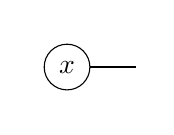
\begin{tikzpicture}[baseline=({N2.base}) ]
            \clip (-0.5,-0.5) rectangle (1,0.5);
            \node[circle, draw] (N2) at (0,0) {$x$};
            \node[] (N1) at (1,0) {};
            \draw  (N1) -- (N2) ;
        \end{tikzpicture}                                                     \\
        M                       & $M_{\alpha \beta}$      & 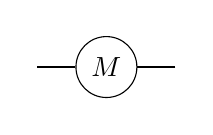
\begin{tikzpicture}[baseline={0cm-0.5*height("$=$")} ]
            \clip (-1,-0.5) rectangle (1,0.5);

            \node[circle, draw] (N2) at (0,0) {$M$};
            \node[] (N0) at (-1,0) {};
            \node[] (N1) at (1,0) {};

            \draw  (N1) -- (N2) ;
            \draw  (N0) -- (N2) ;

        \end{tikzpicture} \\

        $\Vec{x} \cdot \Vec{y}$ & $x_{\alpha} y_{\alpha}$ & 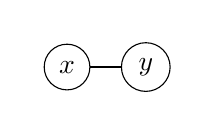
\begin{tikzpicture}[baseline=({N2.base}) ]
            \clip (-0.5,-0.5) rectangle (1.5,0.5);
            \node[circle, draw] (N2) at (0,0) {$x$};
            \node[circle, draw] (N1) at (1,0) {$y$};
            \draw  (N1) -- (N2) ;
        \end{tikzpicture} \\
    \end{tabular}

    \label{tab:grafical_not}
\end{table}

\subsection{Representing a quantum state}

\Glspl{TN} come in many shapes and forms. They are used to represent a tensor with many legs. A general quantum state with N sites can be described in a given basis $\ket{i}$ in the following way:
\begin{equation}
    \ket{\Psi} = \sum_{i_1 i_2 \cdots i_n } C^{i_1 i_2 \cdots i_n} \ket{i_1} \otimes \ket{i_2} \otimes \cdots \otimes \ket{i_n} .
\end{equation}
Here the tensor $C$ holds all the information of the quantum state. The graphical representation can be seen in \cref{fig:tens:intro:C}.
\begin{figure}[!htbp]
    \centering

    \begin{tikzpicture}[ ]

        \draw (-3,-0) rectangle (1,1)  [add reference=C]   ;
        \node  at (C center) {C};

        \node (N1)  at  (-2.5,-1) {};
        \node (N2)  at  (-1.5,-1) {};
        \node  at  (-.5,-0.5) {...};
        \node  (N3) at  (.5,-1) {};

        \draw    (N1) -- (N1 |-  C south);
        \draw    (N2) -- (N2 |-  C south);
        \draw    (N3) -- (N3 |-  C south);

    \end{tikzpicture}

    \caption{Exmple of a tensor C with multiple physical legs.}
    \label{fig:tens:intro:C}
\end{figure}
\noindent
This requires an exponential number $d^n$ of coefficients C where d is the dimension of basis $\ket{i}$. In order to make the problem tractable, the following form is proposed as wave function:
\begin{equation}
    C^{i_1 i_2 \cdots i_n} = {C^{1}}_{\alpha_1}^{ i_1} {C^{2}}_{\alpha_1 \alpha_2}^{i_2} \cdots  {C^{n}}_{\alpha_{n-1} }^{i_n}
\end{equation}

\begin{equation}
    \mpo{4}{{"-",,,,,}}{{"$i_1$","$i_2$",,"$i_n$","-"}}{{"-","-",,"-","-"}}{{0,0,1,0,0}}{{"$C^1$", "$C^2$",,"$C^n$", }}
\end{equation}
where summation over shared indices is implied. It is always possible to find such a representation by means of matrix decomposition (see \cref{sec:mpomath}). The summation bond $\alpha_i$ is called a virtual bond and their dimension is denoted by $\chi$. At this point, this is not yet an improvement because the bond dimension needs to be exponentially large in order to represent the tensor C exactly. To make the chain translation invariant, all the tensors $C^i_{\alpha \beta }$ are the same tensor $C$. The chain is closed by a matrix M which contains the boundary conditions. Setting $\alpha_n = \alpha_0$. We can now write this as a trace over matrix products
\begin{equation}
    \ket{\Psi} = \Tr( C^{i_1} C^{i_2} \cdots C^{i_n} M  ) \ket{i_1} \otimes \ket{i_2} \otimes \cdots \otimes \ket{i_n},
\end{equation}
or in graphical notation
\begin{equation}\label{eq:general_mps}
    \mpo{5}{{"Tr",,,,,}}{{"$i_1$","$i_2$",,"$i_n$","-"}}{{"-","-",,"-","-"}}{{0,0,1,0,0}}{{"C", "C",,"C","M" }} \; .
\end{equation}

\subsection{Classification}

\Glspl{TN} come in many shapes and many forms. During this thesis, we will mainly encounter the types explained here.

\subsubsection{ MPS}

A general \gls{MPS} is of the form \cref{eq:general_mps}. For an infinite extended chain with translation invariance, it is logical to assume a unit cell:
\begin{equation}\label{mps:uni}
    \pepob{5}{2}{{
                "-","-", "-","-",
                "","","",""}}{{
                "-",
                "",
                "",
                "",
                "-"}}{{
                4,4,4,4,4,
                13,0,0,0,13}}
\end{equation}
This will be the form we will work with in this thesis. Of course, larger unit cells are also possible. \Glspl{MPS} are dense. This means that (with a bond dimension exponential in the system size) the \Gls{MPS} can represent every state in the full Hilbert space \cite{Orus2014}. However, the low energy states can typically be represented by a much lower bond dimension. This can be explained in terms of the so-called 'area law': the entropy low energy states often scale with the boundary area of volume. \Glspl{MPS} exactly follow this area law.

\subsubsection{ MPO} \label{mpo_hamil}

Similar to an MPS, a Matrix Product Operator (\Gls{MPO}) is defined by
\begin{equation} \label{def_mpo}
    \begin{split}
        \hat{O} &= \sum Tr(A^{i_1 j_1} A^{i_2 j_2} \cdots A^{i_n j_n} M) \\
        & \times \ket{i_1}\bra{j_1} \otimes \ket{i_2}\bra{j_2} \otimes \cdots \otimes \ket{i_n}\bra{j_n} \\
        &\mpo{5}{{"Tr",,,,,}}{{"$i_1$","$i_2$",,"$i_n$","-"}}{{"$j_1$","$j_2$",,"$j_n$","-"}}{{0,0,1,0,0}}{{"A", "A",,"A","M" }}.
    \end{split}
\end{equation}
The matrix M contains the boundary conditions of the operator. It's clear that this can again be made translationally invariant A uniform \Gls{MPO} is denoted by
\begin{equation}
    \pepob{5}{3}{{
                "-","-", "-","-",
                "","","","",
                "-","-", "-","-",}}{{
                "-","-",
                "","",
                "","",
                "","",
                "-","-",}}{{
                4,4,4,4,4,
                13,0,0,0,13,
                4,4,4,4,4,}}.
\end{equation}
This can also be reinterpreted as an \Gls{MPS} with physical bond dimension $D^2$, by grouping the i and j indices together per site. Acting with an \Gls{MPS} on a \Gls{MPO} $\hat{O} \ket{\Psi} $ again results in an \Gls{MPS}
\begin{equation}
    \vcenter{\hbox{ \pepob{5}{3}{{
                        "-","-", "-","-",
                        "","$\chi$","","",
                        "","$\chi$","","",}}{{
                        "-", "-",
                        "", "",
                        "", "",
                        "", "",
                        "-", "-",}}{{
                        4,4,4,4,4,
                        13,0,0,0,13,
                        13,0,0,0,13}}  }} =   \vcenter{\hbox{ \pepob{5}{2}{{
                        "-","-", "-","-",
                        "","$\chi^2$","",""}}{{
                        "-",
                        "",
                        "",
                        "",
                        "-"}}{{
                        4,4,4,4,4,
                        13,0,0,0,13}} }} \;.
\end{equation}
The new MPS has the same physical dimension, but the bond dimension is increased from $\chi$ to $\chi^2$.

\paragraph{Example of MPO Hamiltonian}

As an example of an MPO representation of a Hamiltonian, consider the \Gls{TFI} Hamiltonian with exponentially decaying interactions:
\begin{equation}
    \hat{H} =  -J   \sum_{j}   \sum_{n>0} \lambda^{n-1} X_j X_{j+n} - h \sum_j Z_j .
\end{equation}
The MPO is
\begin{equation}
    \begin{split}
        \hat{O} &= \begin{bmatrix}
            I    & 0         & 0 \\
            -J X & \lambda I & 0 \\
            -h Z & X         & I
        \end{bmatrix} \\
        \hat{w}_l &= \begin{bmatrix}
            -h Z & X & I \\
        \end{bmatrix} \\
        \hat{w}_r &= \begin{bmatrix}
            I & -J  X & -h Z \\
        \end{bmatrix}^T \\
    \end{split}
\end{equation}
with $X$ and  $Z$ the Pauli matrices, and  $\hat{w}_l$ and  $\hat{w}_l$ the boundary vectors \cite{Zauner-Stauber2018}. Indeed, explicitly performing the multiplication for 3 sites gives
\begin{align}
     & \mpo{3}{{,,,,,}}{{"$i_1$","$i_2$","$i_3$",}}{{"$j_1$","$j_2$","$j_3$",}}{{0,0,0,0,0}}{{ "$w_l$","O","$w_r$" }} \\
     & = \begin{bmatrix}
        -h Z_1 & X_1 & I \\
    \end{bmatrix} \begin{bmatrix}
        I      & 0         & 0 \\
        -J X_2 & \lambda I & 0 \\
        -h Z_2 & X_2       & I
    \end{bmatrix}\begin{bmatrix}
        I       \\
        -J  X_3 \\
        -h Z_3  \\
    \end{bmatrix}                              \\
     & =  \begin{bmatrix}
        ( -h Z_1 - J X_1 X_2 - h Z_2 ) & (- \lambda X_1 + X_2) & I \\
    \end{bmatrix} \begin{bmatrix}
        I       \\
        -J  X_3 \\
        -h Z_3  \\
    \end{bmatrix}                                                       \\
     & = -h ( Z_1 + h Z_2 + h Z_3 ) - J (X_1 X_2+ X_2 X_3 ) - J \lambda X_1 X_3
\end{align}
as expected.

\subsubsection{PEPS}
Projected entangled pair states (\Gls{PEPS}) are the 2D equivalent of \Gls{MPS}. In the visualisation, the physical indices come out of the plane.
\begin{equation}
    \vcenter{ \hbox{ \pepob{5}{5}{{
                        "-","-", "-","-",
                        "",  "", "","",
                        "",  "", "","",
                        "",  "", "","",
                        "-", "-", "-","-",}}{{
                        "-","-", "-","-",
                        "","", "","",
                        "","", "","",
                        "","", "","",
                        "-","-", "-","-",}}{{
                        1,13,13,13,1,
                        13,15,15,15,13,
                        13,15,15,15,13,
                        13,15,15,15,13,
                        1,13,13,13,1,
                    }} }}
\end{equation}
\Glspl{PEPS} also obey the area law, making them efficient parametrisations of the relevant corner of the full Hilbert space.

\subsubsection{PEPO}

The operator version of \Gls{PEPS} is called PEPO. The depiction looks as follows:
\begin{equation}
    \vcenter{ \hbox{ \pepob{5}{5}{{
                        "-","-", "-","-",
                        "",  "", "","",
                        "",  "", "","",
                        "",  "", "","",
                        "-", "-", "-","-",}}{{
                        "-","-", "-","-",
                        "","", "","",
                        "","", "","",
                        "","", "","",
                        "-","-", "-","-",}}{{
                        1,13,13,13,1,
                        13,14,14,14,13,
                        13,14,14,14,13,
                        13,14,14,14,13,
                        1,13,13,13,1,
                    }} }}
\end{equation}

\subsubsection{Others}

To show there exist many more \Glspl{TN} beside the ones treated in this thesis, 2 examples are shown in \cref{fig:tnalgs:ttn_mera}. Two Tree Tensor Networks (TTNs)  are shown. The red indices are physical. multi-scale entanglement renormalization ansatz (MERA) (c) is also shown. These \Glspl{TN} are special because they can be contracted exactly, as opposed to for instance \Gls{PEPS}.

\begin{figure}[!htbp]
    \center
    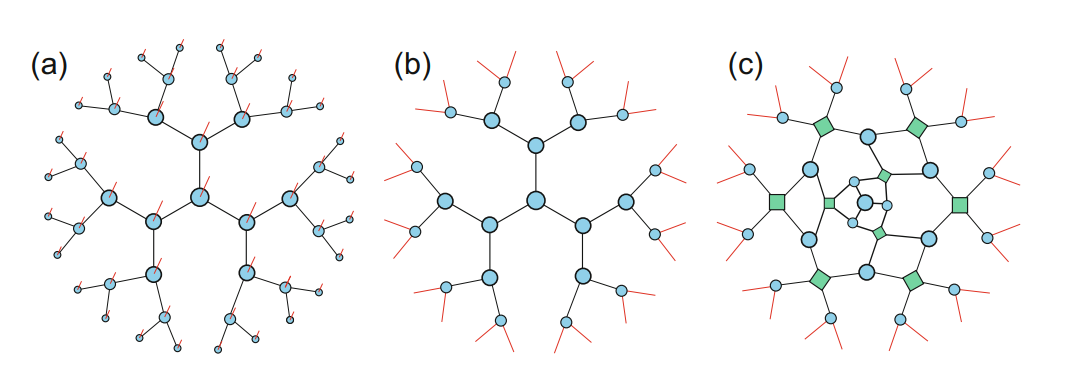
\includegraphics[width=0.8 \textwidth]{Figuren/tnalgs/tnns_and_mera.png}
    \caption{ (a) and (b) two different TTNSs and (c) MERA. Figure taken from \cite{Ran2020}.  }
    \label{fig:tnalgs:ttn_mera}
\end{figure}

%https://link.springer.com/content/pdf/10.1007%2F978-3-030-34489-4.pdf